\documentclass[border=0]{standalone}
\usepackage{booktabs}
\usepackage{tikz}

\usetikzlibrary{positioning}

\begin{document}
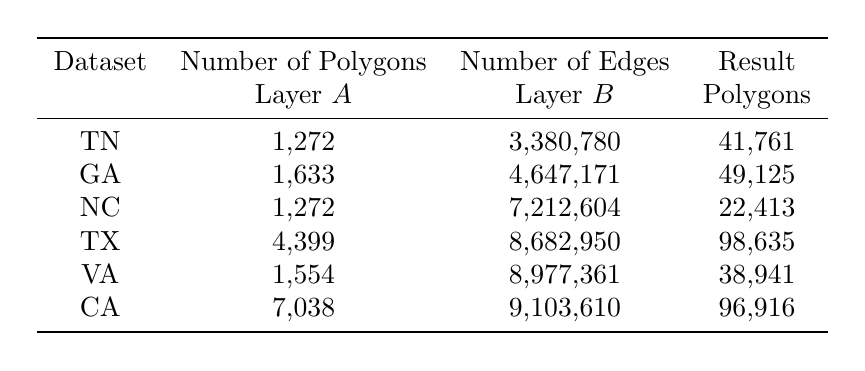
\begin{tikzpicture}
    \node[] (vertices) at (0,0) {
        \begin{tabular}{c c c c}
            \toprule
            Dataset & Number of Polygons    & Number of Edges   & Result    \\
                    & Layer $A$             & Layer $B$         & Polygons  \\
            \midrule
            TN & 1,272 & 3,380,780 & 41,761 \\
            GA & 1,633 & 4,647,171 & 49,125 \\
            NC & 1,272 & 7,212,604 & 22,413 \\
            TX & 4,399 & 8,682,950 & 98,635 \\
            VA & 1,554 & 8,977,361 & 38,941 \\
            CA & 7,038 & 9,103,610 & 96,916 \\
            \bottomrule
        \end{tabular}
    };
\end{tikzpicture}
\end{document}
